\documentclass{article}

% Chinese Support using xeCJK
% \usepackage{xeCJK}
% \setCJKmainfont{SimSun}

% Chinese Support using CTeX
% \usepackage{ctex}

% Math Support
\usepackage{amsmath}
\usepackage{amsfonts}
\usepackage{amssymb}
\usepackage{wasysym}

% Graphics Support
\usepackage{graphicx}
\usepackage{float}

% Reduced page margin
\usepackage{geometry}
\geometry{a4paper,scale=0.8}

\usepackage{caption}
\usepackage{subcaption}

% d and e should be math operators
\newcommand*{\dif}{\mathop{}\!\mathrm{d}}
\newcommand*{\md}{\mathop{}\!\mathrm{d}}
\newcommand*{\me}{\mathrm{e}}

% No indent for each paragraph
\usepackage{parskip}
\setlength{\parindent}{0cm}

% Bold style for Greek letters
\usepackage{bm}
\let\Oldmathbf\mathbf
\renewcommand{\mathbf}[1]{\boldsymbol{\Oldmathbf{#1}}}

% More space for dfrac in cell
\usepackage{cellspace}
\setlength{\cellspacetoplimit}{5pt}
\setlength{\cellspacebottomlimit}{5pt}

% SI units
\newcommand{\si}[1]{\  \mathrm{#1}}

% Multi-line author information
\usepackage{authblk}
\author{Xiping Hu}
\affil{https://hxp.plus/}

\title{Homework for Chapter 10}

\begin{document}

\maketitle

\begin{figure}[H]
  \centering
  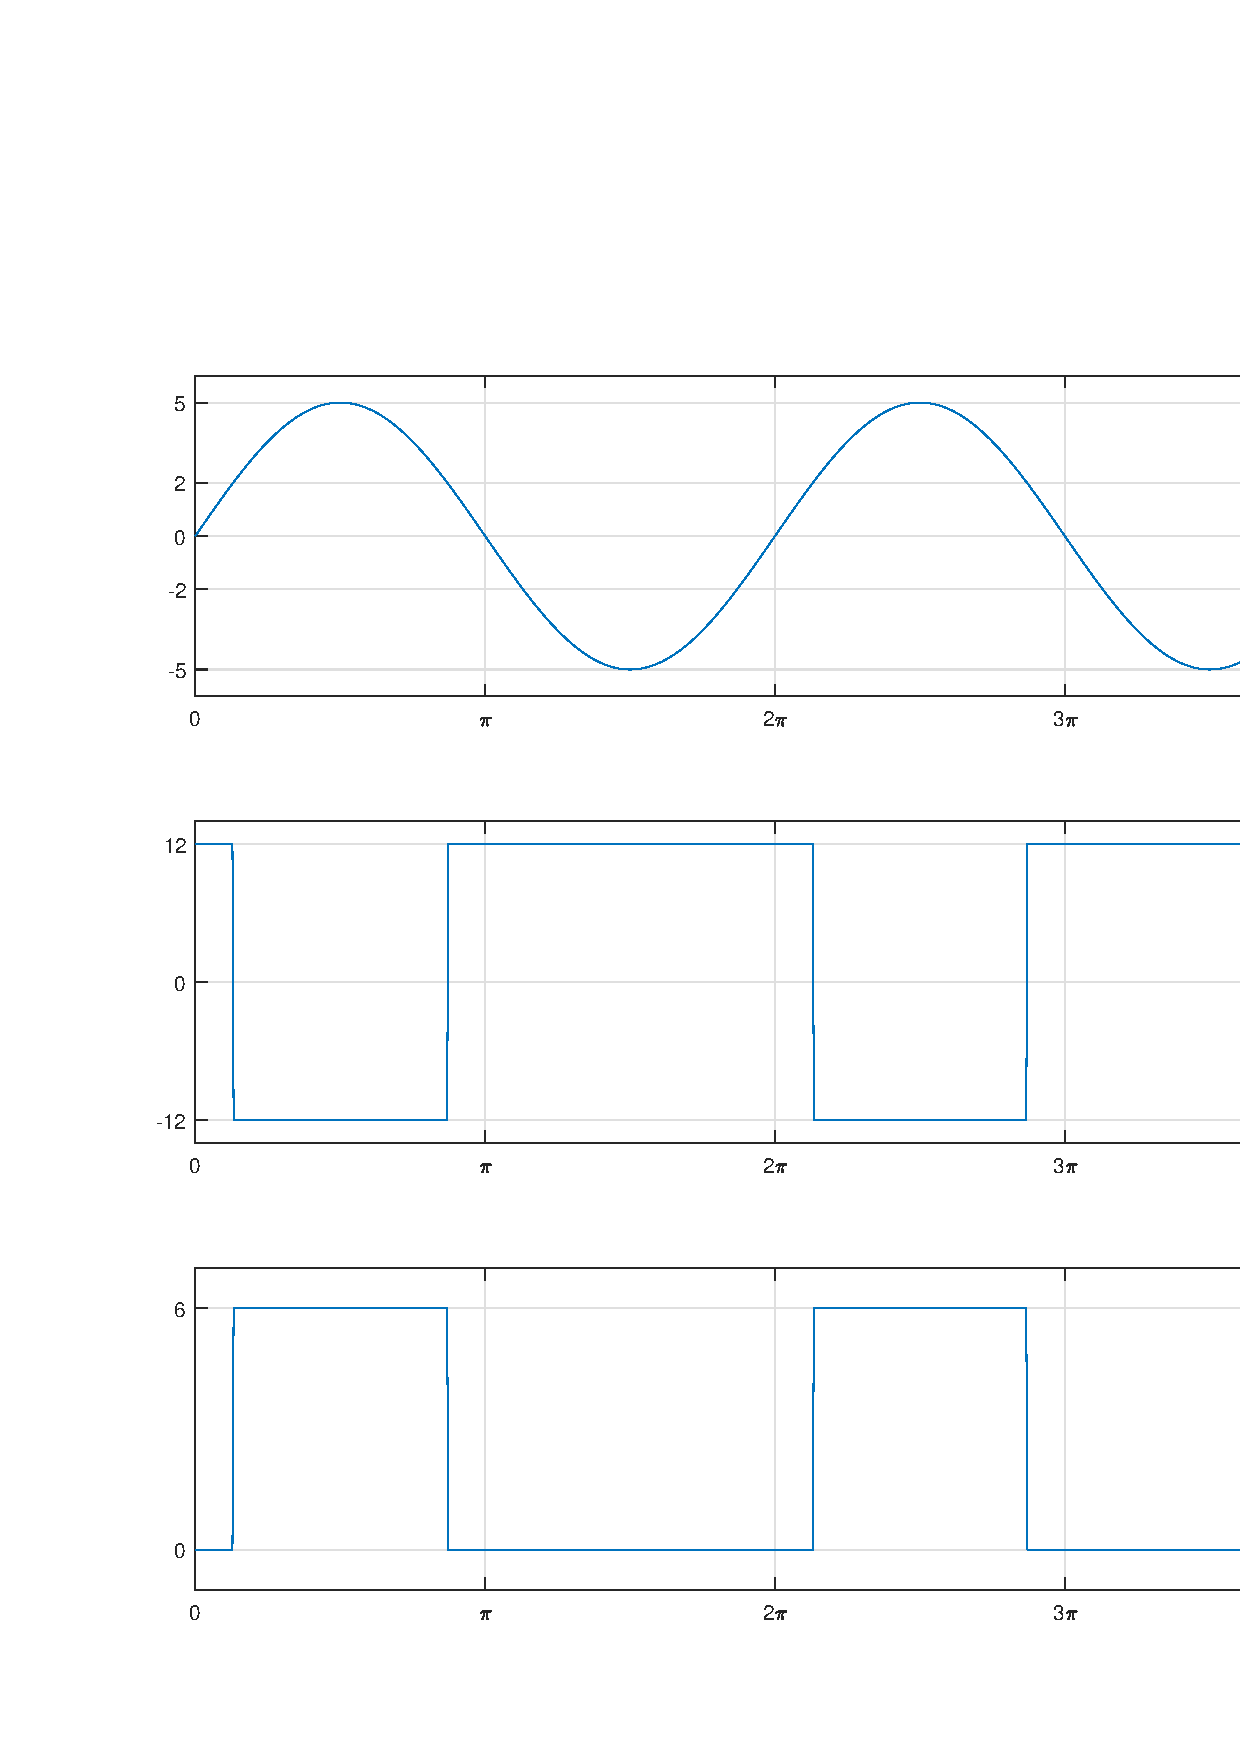
\includegraphics[width=\linewidth]{figures/Problem1081.png}
\end{figure}

\section{Problem 1}

\begin{equation*}
  \begin{aligned}
    v_{o1} = 1 \si{V} \quad v_{o2} = 12 \si{V} \quad I_B = \dfrac{12 \si{V}}{51 \si{k \Omega}} = 235.3 \si{\mu A}
  \end{aligned}
\end{equation*}

\begin{equation*}
  \begin{aligned}
    I_{BS} = \dfrac{6 \si{V}}{R_c \beta} = 23.5 \si{\mu A} \quad \ll \quad I_B = 235.3 \si{\mu A} \quad \Rightarrow \quad v_o = 0 \si{V}
  \end{aligned}
\end{equation*}

\section{Problem 2}

\begin{equation*}
  \begin{aligned}
    v_1 = 3 \si{V} \quad v_{o1} = 3 \si{V} \quad v_{o2} = - 12 \si{V} \quad v_o = 6 \si{V}
  \end{aligned}
\end{equation*}

\section{Problem 3}

\begin{figure}[H]
  \centering
  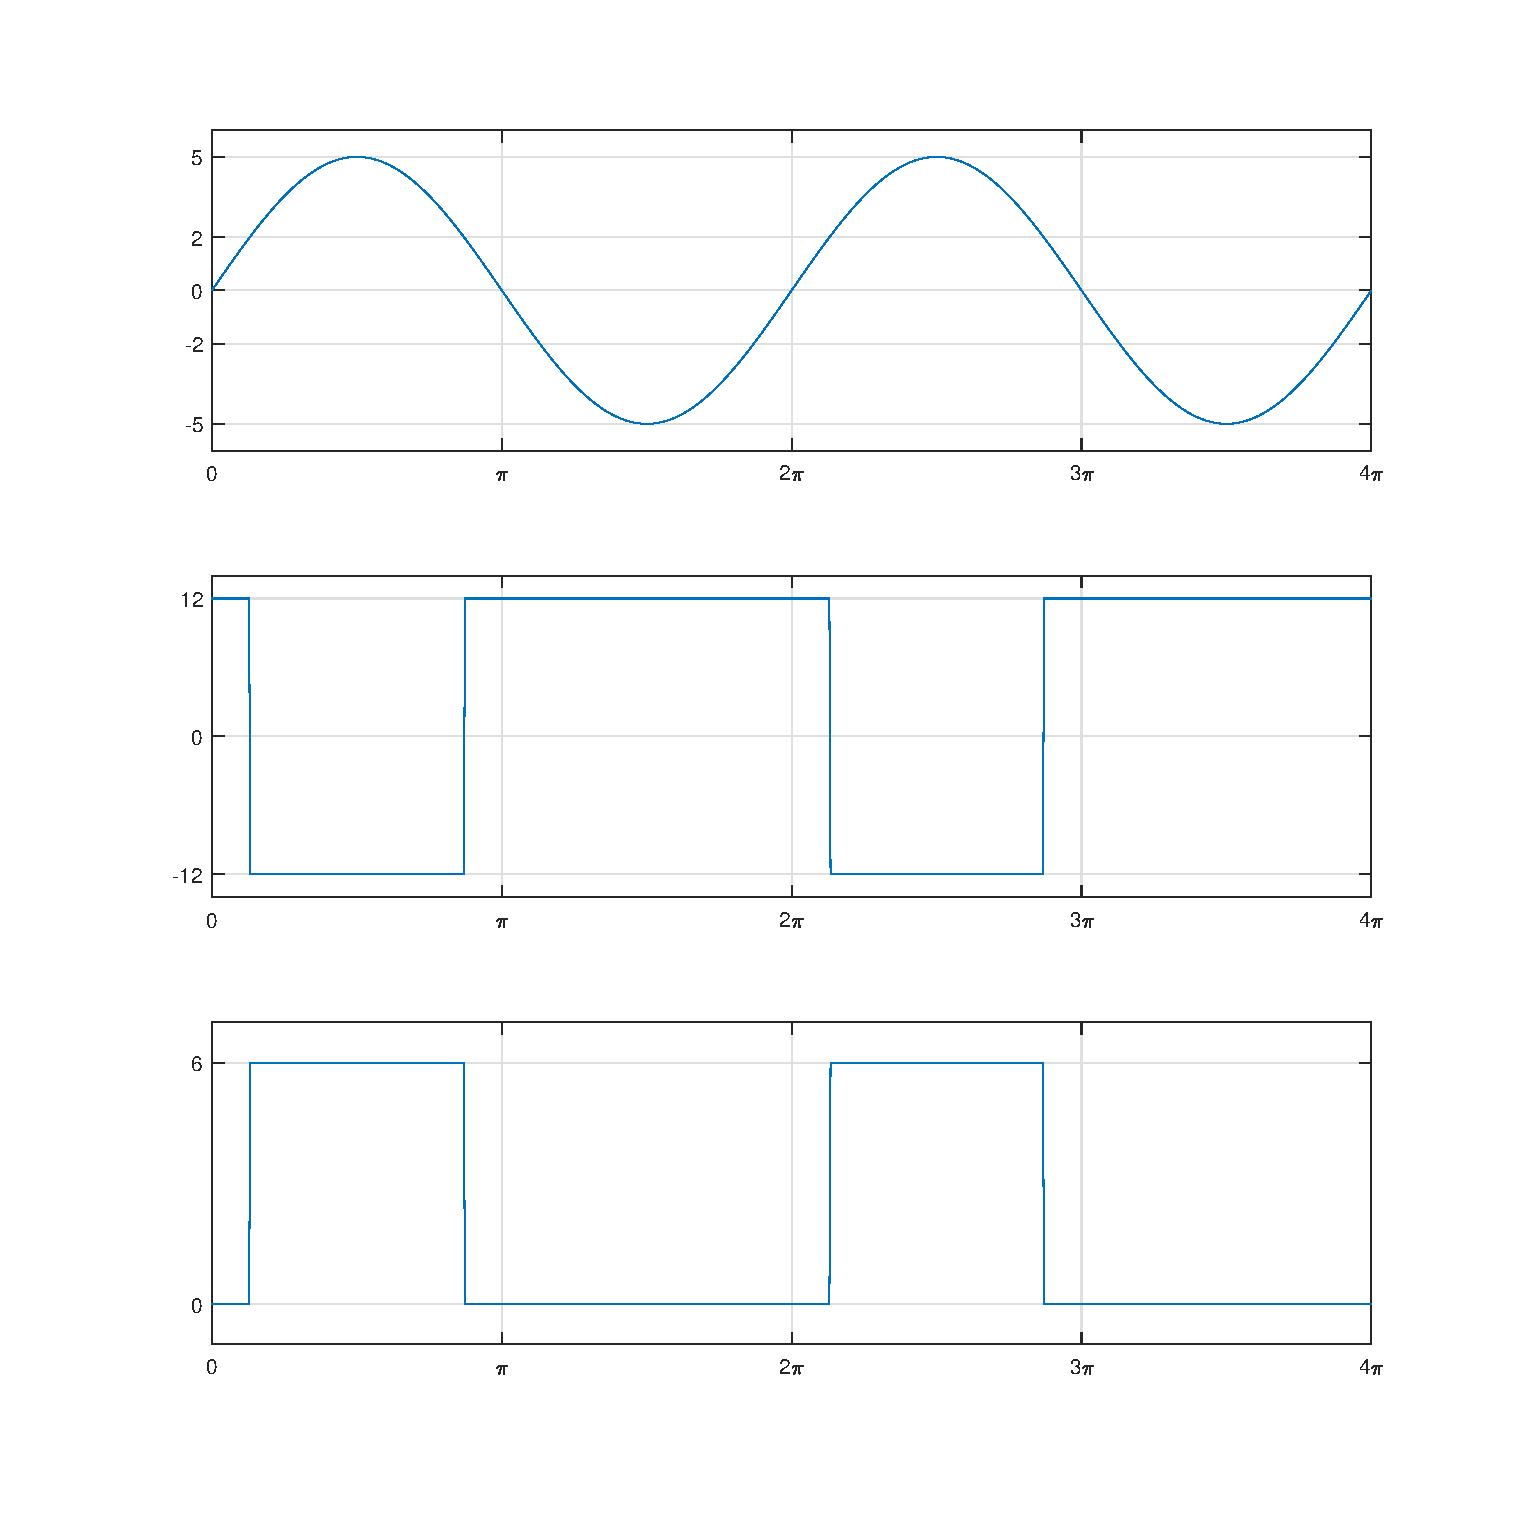
\includegraphics[width=\linewidth]{figures/Problem1081.eps}
\end{figure}

\end{document}